% !TeX root = surprises.tex

\chapter{Un compás es suficiente}\label{c.compass}

%%%%%%%%%%%%%%%%%%%%%%%%%%%%%%%%%%%%%%%%%%%%%%%%%%%%%%%%%%%%%%%

\index{Construction!compass@with only a compass|(}
En 1797 Lorenzo Mascheroni demostró que cualquier construcción realizada con regla y compás puede realizarse sólo con compás. Más tarde se supo que este teorema ya había sido demostrado por Georg Mohr en 1672.
Después de explicar en Sec.~\ref{s.compass-what} lo que se entiende por la realización de una construcción con sólo un compás, la demostración se presenta en etapas a partir de cuatro construcciones auxiliares: la reflexión de un punto (Sec.~\ref{s.reflection}), la construcción de un círculo con un radio dado (Sec.~\ref{s.circle}), suma y resta de segmentos (Sec.~\ref{s.add-subtract}) y construcción de un segmento como cociente de segmentos (Sec.~\ref{s.three}). La sección~\ref{s.two-lines} muestra cómo encontrar la intersección de dos líneas y la sección~\ref{s.line-circle} muestra cómo encontrar la intersección de una línea y un círculo.

\section{¿Qué es una construcción con sólo un compás?}\label{s.compass-what}

Figura~\ref{f.compass-equi} muestra la construcción de un triángulo equilátero utilizando una regla y un compás. ¿Cómo podemos construir un triángulo sin los segmentos $\overline{AB}, \overline{AC}, \overline{BC}$? Un segmento está definido por dos puntos, por lo que basta con construir estos puntos para obtener una construcción equivalente a la realizada con regla (Fig.~\ref{f.compass-equi-only}). No es necesario \emph{ver} realmente los segmentos.
Habrá líneas en las figuras de este capítulo, pero se utilizan sólo para entender la construcción y la demostración de su exactitud. Es importante convencerse de que la construcción en sí utiliza sólo un compás.

\begin{figure}%[b]
\begin{minipage}{.45\textwidth}
\begin{center}
\begin{tikzpicture}[scale=0.6]
\coordinate (A) at (0,0);
\coordinate (B) at (4,0);
\vertex{A};
\vertex{B};
\draw (A) node[below left] {$A$} -- (B) node[below right] {$B$};
\draw[name path=larc] (A) ++(-10:4cm) arc (-10:80:4cm);
\draw[name path=rarc] (B) ++(-170:4cm) arc (-170:-260:4cm);
\path [name intersections={of=larc and rarc,by={t}}];
\node[above right,xshift=-2pt,yshift=3pt] at (t) {$C$};
\vertex{t};
\draw (A) -- (t);
\draw (B) -- (t);
\end{tikzpicture}
\caption{Construcción de un triángulo equilátero con regla y compás}\label{f.compass-equi}
\end{center}
\end{minipage}
\hfill
\begin{minipage}{.45\textwidth}
\begin{center}
\begin{tikzpicture}[scale=0.6]
\coordinate (A) at (0,0);
\coordinate (B) at (4,0);
\vertex{A};
\vertex{B};
\path (A) node[below left] {$A$} -- (B) node[below right] {$B$};
\draw[name path=larc] (A) ++(-10:4cm) arc (-10:80:4cm);
\draw[name path=rarc] (B) ++(-170:4cm) arc (-170:-260:4cm);
\path [name intersections={of=larc and rarc,by={t}}];
\node[above right,xshift=-2pt,yshift=3pt] at (t) {$C$};
\vertex{t};
\end{tikzpicture}
\caption{Construcción de un triángulo equilátero con sólo un compás}\label{f.compass-equi-only}
\end{center}
\end{minipage}
\end{figure}

Una construcción con regla y compás es una secuencia de tres operaciones:
\begin{itemize}
\item Hallar el punto de intersección de dos rectas.
\item Hallar el punto o puntos de intersección de una recta y una circunferencia.
\item Hallar el punto o puntos de intersección de dos circunferencias.
\end{itemize}
La tercera operación se puede hacer sólo con un compás. Tenemos que demostrar que las dos primeras operaciones se pueden hacer sólo con un compás.

\noindent{}Notation:
\begin{itemize}
\item $c(O,A)$: la circunferencia con centro $O$ que pasa por el punto $A$.
\item $c(O,r)$: la circunferencia con centro $O$ y radio $r$.
\item $c(O,\overline{AB})$: la circunferencia con centro $O$ y radio la longitud del segmento $\overline{AB}$.
\end{itemize}

%%%%%%%%%%%%%%%%%%%%%%%%%%%%%%%%%%%%%%%%%%%%%%%%%%%%%%%%%%%%%%%

\section{Reflexión de un punto}\label{s.reflection}

\begin{definition}
Un punto $C'$ es un \emph{reflejo} del punto $C$ alrededor de un segmento $\overline{AB}$ si y sólo si $\overline{AB}$ (o la recta que contiene a $\overline{AB}$) es la mediatriz del segmento $\overline{CC'}$.
\end{definition}

\begin{theorem}\label{thm.compass-reflection}
Dada una recta $\overline{AB}$ y un punto $C$ que no está en $\overline{AB}$, es posible construir $C'$, la reflexión de $C$ alrededor de $\overline{AB}$.
\end{theorem}

\begin{figure}%[b]
\begin{center}
\begin{tikzpicture}[scale=.7]
\coordinate (A) at (0,0);
\coordinate (B) at (4,0);
\coordinate (C) at (2.5,1.5);
\draw ($(B)!2!(A)$) -- ($(A)!2!(B)$);
\node[above left] at (A) {$A$};
\node[above right] at (B) {$B$};
\node[above,yshift=4pt] at (C) {$C$};
\node[draw,circle through=(C),name path=ac] at (A) {};
\node[draw,circle through=(C),name path=bc] at (B) {};
\path [name intersections={of=ac and bc,by={x1,Cp}}];
\node[below,yshift=-4pt] at (Cp) {$C'$};
\draw (C) -- (Cp);
\vertex{A};
\vertex{B};
\draw (A) -- (C);
\draw (B) -- (C);
\draw (A) -- (Cp);
\draw (B) -- (Cp);
\coordinate (center) at (2.5,0);
\draw[rotate=90] (center) rectangle +(8pt,8pt);
\end{tikzpicture}
\end{center}
\caption{Construcción de un reflejo}\label{f.compass-reflection}
\end{figure}

\begin{proof} 
Construimos una circunferencia centrada en $A$ que pase por $C$ y una circunferencia centrada en $B$ que pase por $C$. La otra intersección de las dos circunferencias es el punto $C'$ que es la reflexión de $C$ (Fig.~\ref{f.compass-reflection}).
$\triangle ABC \cong \triangle ABC'$ por lado-lado ya que $\overline{AC}, \overline{AC'}$ son radios de la misma circunferencia, al igual que $\overline{BC}, \overline{BC'}$ y $\overline{AB}$ es un lado común. Por lo tanto, $\angle CAB = \angle C'AB$ por lo que $\overline{AB}$ es la bisectriz del ángulo $\angle CAC'$. Pero $\triangle CAC'$ es un triángulo isósceles y la bisectriz del ángulo $\overline{AB}$ es también la mediatriz de $\overline{CC'}$, la base de $\triangle CAC'$. Por definición $C'$ es la reflexión de $C$ alrededor de $\overline{AB}$.
\end{proof}

\begin{figure}%[t]
\begin{center}
\begin{tikzpicture}[scale=.5]
\coordinate (A) at (0,1.5);
\coordinate (B) at (0,-1.5);
\coordinate (C) at (1.5,-3);
\coordinate (Cp) at (1.5,3);
\vertex{A};
\vertex{B};
\vertex{C};
\node[above] at (A) {$A$};
\node[below] at (B) {$B$};
\node[below] at (C) {$C$};
\node[draw,circle through=(B),name path=ab] at (A) {};
\node[draw,circle through=(A),name path=ba] at (B) {};
\path [name intersections={of=ab and ba,by={Y,X}}];
\node[above right,xshift=4pt] at (X) {$X$};
\node[above left,xshift=-4pt] at (Y) {$Y$};
\draw[dashed] ($(X)!2!(Y)$) -- ($(Y)!2!(X)$);
\coordinate (Cp) at (1.5,3);
\vertex{Cp};
\node[above,yshift=2pt] at (Cp) {$C'$};
\draw (A) -- (B);
\draw (C) -- (Cp);
\draw (Y) -- (A) -- (X) -- (B) -- cycle;
\end{tikzpicture}
\end{center}
\caption{Construcción de un círculo de radio determinado (1)}\label{f.compass-circle1}
\end{figure}
%%%%%%%%%%%%%%%%%%%%%%%%%%%%%%%%%%%%%%%%%%%%%%%%%%%%%%%%%%%%%%%

\section{Construcción de un círculo de radio dado}\label{s.circle}

\begin{theorem}\label{thm.compass-radius}
Dados los puntos $A,B,C$ es posible construir $c(A,\overline{BC})$, la circunferencia centrada en $A$ con radio $\overline{BC}$.
\end{theorem}

\begin{proof}
Construimos $c(A,B)$ y $c(B,A)$ y tal que $X$, $Y$ son sus puntos de intersección (Fig.~\ref{f.compass-circle1}). $A$ es el reflejo de $B$ alrededor de $\overline{XY}$ ya que $\triangle YAX\cong \triangle YBX$ porque tienen sus tres lados correspondientes iguales. Por el Teorema~\ref{thm.compass-reflection} construimos $C'$, el reflejo de $C$ alrededor de $\overline{XY}$ y luego construimos $c(A,\overline{AC'})$ (Fig.~\ref{f.compass-circle3}).


\begin{figure}%
\begin{center}
\begin{tikzpicture}[scale=.6]
\coordinate (A) at (0,1.5);
\coordinate (B) at (0,-1.5);
\coordinate (C) at (1.5,-3);
\coordinate (Cp) at (1.5,3);
\node[above,yshift=2pt] at (A) {$A$};
\node[below,yshift=-2pt] at (B) {$B$};
\node[below,yshift=-2pt] at (C) {$C$};
\node[above,xshift=1pt,yshift=2pt] at (Cp) {$C'$};
\node[circle through=(B),name path=ab] at (A) {};
\node[circle through=(A),name path=ba] at (B) {};
\path [name intersections={of=ab and ba,by={Y,X}}];
\node[above right,xshift=4pt] at (X) {$X$};
\node[above left,xshift=-4pt] at (Y) {$Y$};
%\node[draw,circle through=(C)] at (Y) {};
\draw[dashed] ($(X)!1.8!(Y)$) -- ($(Y)!1.8!(X)$);
\path[name path=xy] (X) -- (Y);
\node[draw,thick,circle through=(Cp)] at (A) {};
\draw (A) -- (Cp);
\draw (B) -- (C);
\draw[name path=abline] (A) -- (B);
\draw[name path=ccp] (C) -- (Cp);
\path[name intersections={of=xy and abline,by={D}}];
\path[name intersections={of=xy and ccp,by={E}}];
\node[above left] at (D) {$D$};
\node[below right,xshift=-3pt] at  (E) {$E$};
\draw (D) -- (Cp);
\draw (D) -- (C);
\draw (D) rectangle +(9pt,9pt);
\draw (E) rectangle +(9pt,9pt);
\vertex{Y};
\vertex{A};
\vertex{X};
\end{tikzpicture}
\end{center}
\caption{Construcción de un círculo de radio determinado (2)}\label{f.compass-circle3}
\end{figure}

$\overline{XY}$ es la mediatriz de $\overline{CC'}$ y $\overline{AB}$. Denotemos con $D$ a la intersección de $\overline{XY}$ y $\overline{AB}$ y con $E$ la intersección de $\overline{XY}$ y $\overline{CC'}$. Entonces $\overline{C'E}=\overline{EC}$, $\overline{AD}=\overline{DB}$ y $\angle DEC=\angle DEC'$ es un ángulo recto, por lo que $\triangle DEC\cong\triangle DEC'$ por lado-ángulo-lado. Por tanto, $\overline{DC}=\overline{DC'}$ y $\angle ADC'=\angle BDC$ (son complementarios de $\angle EDC'=\angle EDC$). Se deduce que $\triangle ADC'\cong\triangle BDC$ por lado-ángulo-lado por lo que $\overline{AC'}=\overline{BC}$.
\end{proof}

%%%%%%%%%%%%%%%%%%%%%%%%%%%%%%%%%%%%%%%%%%%%%%%%%%%%%%%%%%%%%%%

\section{Suma y resta de segmentos}\label{s.add-subtract}

\begin{theorem}\label{thm.add-subtract-mm}
Dado un segmento $\overline{PQ}$ de longitud $a$ y un segmento $\overline{RS}$ de longitud $b$, es posible construir segmentos $\overline{QT}, \overline{QU}$ tales que $\overline{PTQU}$ es un segmento, la longitud de $\overline{PT}$ es $a-b$ y la longitud de $\overline{PU}$ es $a+b$ (Fig.~\ref{f.compass-add1}).
\end{theorem}
\begin{figure}%
\begin{center}
\begin{tikzpicture}[scale=.8]
\coordinate (P) at (0,0);
\coordinate (Q) at (5,0);
\coordinate (T) at (3,0);
\coordinate (U) at (7,0);
\vertex{P};
\vertex{Q};
\vertex{U};
\vertex{T};
\draw (P) -- (Q);
\node[above] at (P) {$P$};
\node[above left] at (Q) {$Q$};
\node[above left] at (U) {$U$};
\node[above right] at (T) {$T$};
\draw (5,0) -- (8,0);
\coordinate (R) at (9,-1);
\coordinate (S) at ($(9,-1) + (20:2cm)$);
\vertex{R};
\vertex{S};
\draw (R) node[above] {$R$} -- node[below right] {$b$} (S) node[above] {$S$};
\draw[<->] (0,-.5) -- node[fill=white] {$a$} (5,-.5);
\draw[<->] (0,-1) -- node[fill=white] {$a-b$} (3,-1);
\draw[<->] (0,-1.5) -- node[fill=white] {$a+b$} (7,-1.5);
\end{tikzpicture}
\end{center}
\caption{Suma y resta de segmentos}\label{f.compass-add1}
\end{figure}

La demostración es bastante larga y se presentará como una secuencia de construcciones.

\begin{theorem}\label{thm.compass-trapezoid}
Se puede construir un trapecio isósceles.
\end{theorem}

\begin{figure}%[b]
\begin{center}
\begin{tikzpicture}[scale=.5]
\coordinate (Q) at (0,0);
\coordinate (P) at (-6.8,0);
\coordinate (B) at (-3,-2);
\draw ($(Q)!1.3!(P)$) -- node[above,near start] {$a$} ($(P)!2.3!(Q)$);
\node[above left] at (Q) {$Q$};
\node[above] at (P) {$P$};
\node[draw,circle through=(B),name path=qb] at (Q) {};
\draw (Q) -- node[left,xshift=-1pt,yshift=2pt] {$b$} (B);
\path[name path=qh] (Q) -- (-40:5cm);
\path[name path=qhp] (Q) -- (40:5cm);
\path [name intersections={of=qb and qh,by={H}}];
\path [name intersections={of=qb and qhp,by={Hp}}];
\node[right,xshift=2pt] at (H) {$H'$};
\node[right,xshift=2pt] at (Hp) {$H$};
\draw (H) -- node[below left,yshift=-2pt] {$h$} (Hp);
\vertex{P};
\vertex{Q};
\end{tikzpicture}
\end{center}
\caption{Construcción de un trapecio isósceles (1)}\label{f.compass--trap1}
\end{figure}

\begin{figure}%
\begin{center}
\begin{tikzpicture}[scale=.5]
\coordinate (Q) at (0,0);
\coordinate (P) at (-6.8,0);
\coordinate (B) at (-3,-2);
\draw ($(Q)!1.3!(P)$) -- ($(P)!2.3!(Q)$);
\vertex{Q};
\vertex{P};
\node[above right,xshift=7pt] at (Q) {$Q$};
\node[above] at (P) {$P$};
\node[draw,circle through=(B),name path=qb] at (Q) {};
\draw (Q) -- node[left,xshift=-1pt,yshift=2pt] {$b$} (B);
\path[name path=qh] (Q) -- (-40:5cm);
\path[name path=qhp] (Q) -- (40:5cm);
\path [name intersections={of=qb and qh,by={Hp}}];
\path [name intersections={of=qb and qhp,by={H}}];
\node[right,xshift=2pt] at (H) {$H$};
\node[right,xshift=2pt] at (Hp) {$H'$};
\draw (H) -- node[below left,yshift=-3pt] {$h$} (Hp);
\vertex{H};
\coordinate (Qp) at (H|-Q);
\draw (Qp) rectangle +(10pt,10pt);
\node[above left] at (Qp) {$Q'$};
\draw[name path=circleqh] (Q) let
  \p1 = ($ (H) - (Hp) $),
  \n2 = {veclen(\x1,\y1)}
in
  circle (\n2)
  (Q) edge node[below] {$h$} +(140:\n2) ++(140:\n2) coordinate (q);
\draw[name path=circlehb] (H) let
  \p1 = ($ (Q) - (B) $),
  \n2 = {veclen(\x1,\y1)}
in
  circle (\n2)
  (H) edge node[below,near end] {$b$} +(50:\n2) ++(50:\n2)  coordinate (h);
\path [name intersections={of=circleqh and circlehb,by={K}}];
\node[above left] at (K) {$K$};
\draw let
  \p1 = ($ (K) - (Q) $)
in
  coordinate (Kp) at (\x1,-\y1);
\node[below left] at (Kp) {$K'$};
\draw (K) -- (Kp);
\draw (Q) rectangle +(10pt,10pt);
\draw[dashed] (K) -- node[right,yshift=1pt] {$b$} (H) -- (Q);
\draw[dashed] (Kp) -- (Hp) -- (Q);
\end{tikzpicture}
\end{center}
\caption{Construcción de un trapecio isósceles (2)}\label{f.compass--trap2}
\end{figure}

\begin{figure}%[ht]
\begin{center}
\begin{tikzpicture}[scale=.5]
\coordinate (Q) at (0,0);
\coordinate (P) at (-6.8,0);
\coordinate (B) at (-3,-2);
\draw[dashed] ($(Q)!1.3!(P)$) -- ($(P)!2.3!(Q)$);
\node[above left] at (Q) {$Q$};
\node[above] at (P) {$P$};
\vertex{P};
\vertex{Q};
\node[draw,circle through=(B),name path=qb] at (Q) {};
\path[name path=qh] (Q) -- (-40:5cm);
\path[name path=qhp] (Q) -- (40:5cm);
\path [name intersections={of=qb and qh,by={Hp}}];
\path [name intersections={of=qb and qhp,by={H}}];
\node[right,xshift=2pt] at (H) {$H$};
\node[right,xshift=2pt] at (Hp) {$H'$};
\draw (H) -- node[below right,yshift=-2pt] {$h$} (Hp);
\path[name path=circleqh] (Q) let
  \p1 = ($ (H) - (Hp) $)
in
  circle ({veclen(\x1,\y1)});
\path[name path=circlehb] (H) let
  \p1 = ($ (Q) - (B) $)
in
  circle ({veclen(\x1,\y1)});
\path [name intersections={of=circleqh and circlehb,by={K,k2}}];
\node[above left] at (K) {$K$};
\draw (Q) -- node[left] {$h$} (K);
\draw (H) -- node[right,xshift=4pt] {$b$} (K);
\draw let
  \p1 = ($ (K) - (Q) $)
in
  coordinate (Kp) at (\x1,-\y1);
\node[below left] at (Kp) {$K'$};
\draw (Q) -- node[left] {$h$} (Kp) -- node[right,xshift=2pt,yshift=-2pt] {$b$} (Hp);
\draw (K) -- node[above right] {$d$} (Hp);
\draw (Kp) -- node[left] {$d$} (H);
\end{tikzpicture}
\end{center}
\caption{Construcción de un trapecio isósceles (3)}\label{f.compass--trap3}
\end{figure}

\begin{proof}
Sea $H$ un punto cualquiera sobre $c(Q,b)$. Construimos $H'$ su reflexión en torno a $\overline{PQ}$. Denotemos la longitud de $\overline{HH'}$ por $h$  (Fig.~\ref{f.compass--trap1}). Construimos las circunferencias $c(H,b)$, $c(Q,h)$. Sea $K$ un punto de intersección de las circunferencias y construyamos $K'$ la reflexión de $K$ en torno a $\overline{PQ}$ (Fig.~\ref{f.compass--trap2}).
La recta que contiene $\overline{PQ}$ es la mediatriz de $\overline{HH'}$ y $\overline{KK'}$ por lo que $\overline{HH'}\parallel\overline{KK'}$. $\overline{KH}=b$ ya que es el radio de la circunferencia centrada en $H$, y $K',H'$ son reflexiones de $K,H$. $\triangle QQ'H\cong \triangle QQ'H'$ por lado-ángulo-lado y $\triangle KQH\cong \triangle K'QH'$ por lado-lado-lado, por lo que $\overline{K'H'}=\overline{KH}=b$. Resulta que $\overline{KHH'K'}$ es un trapecio isósceles cuyas bases son $\overline{HH'}=h$, $\overline{KK'}=2h$ (Fig.~\ref{f.compass--trap3}). Denotemos por $d$ la longitud de las diagonales $\overline{K'H}=\overline{KH'}$.
\end{proof}
\begin{figure}%[h]
\begin{center}
\begin{tikzpicture}[scale=.5]
\coordinate (Q) at (0,0);
\coordinate (P) at (-6.8,0);
\coordinate (B) at (-3,-2);
\draw[name path=pq] ($(Q)!1.3!(P)$) -- ($(P)!2.3!(Q)$);
\node[above left] at (Q) {$Q$};
\node[above] at (P) {$P$};
\node[draw,circle through=(B),name path=qb] at (Q) {};
\path[name path=qh] (Q) -- (-40:5cm);
\path[name path=qhp] (Q) -- (40:5cm);
\path [name intersections={of=qb and qh,by={hp}}];
\path [name intersections={of=qb and qhp,by={H}}];
\node[right,xshift=2pt] at (H) {$H$};
\node[right,xshift=2pt] at (hp) {$H'$};
\draw (H) -- (hp);
\path[name path=circleqh] (Q) let
  \p1 = ($ (H) - (hp) $)
in
  circle ({veclen(\x1,\y1)});
\path[name path=circlehb] (H) let
  \p1 = ($ (Q) - (B) $)
in
  circle ({veclen(\x1,\y1)});
\path [name intersections={of=circleqh and circlehb,by={K,k2}}];
\node[above left] at (K) {$K$};
\draw (Q) -- (K);
\draw (H) -- (K);
\draw let
  \p1 = ($ (K) - (Q) $)
in
  coordinate (kp) at (\x1,-\y1);
\node[below left] at (kp) {$K'$};
\draw (Q) -- node[left] {$h$} (kp) -- (hp);
\draw (K) -- (hp);
\draw (kp) -- (H);
\path [name intersections={of=pq and qb,by={X,x2}}];
\node[below right] at (X) {$X$};
\draw (kp) -- node[right] {$x$} (X);
\draw[very thick] (Q) -- (kp) -- (X) -- node[above,xshift=-8pt] {$b$} cycle;
\vertex{P};
\vertex{Q};
\end{tikzpicture}
\end{center}
\caption{Aplicación del teorema de Ptolomeo}\label{f.compass--trap4}
\end{figure}

\begin{theorem}
Un trapecio  puede estar inscrito en una circunferencia.
\end{theorem}

\begin{proof}
El teorema se deduce inmediatamente de Teoremas.~\ref{thm.quad-circum} y ~\ref{thm.-trapezoid}.
\end{proof}

\begin{theorem}\label{thm.ptolemy-trap}
Para $d,b,h$ mostrados en la figura~\ref{f.compass--trap3}, $d^2=b^2+2h^2$.
\end{theorem}

\begin{proof}
El teorema se deduce del teorema de Ptolomeo (Teorema~\ref{thm.ptolemy}) que dice que en un cuadrilátero inscrito en una circunferencia el producto de las diagonales es igual a la suma de los productos de los lados opuestos.
\end{proof}

Ahora se puede dar la demostración de Teorema~\ref{thm.add-subtract-mm}.
\begin{proof}
Sea $X$ el punto de la recta $\overline{PQ}$ que prolonga $\overline{PQ}$ por $b$. (Eventualmente construiremos $X$.) Definir $x = \overline{K'X}$. En el Teorema~\ref{thm.ptolemy-trap}:
\[
d^2=b^2 + 2h^2 = (x^2-h^2)+2h^2 =x^2+h^2\,.
\]
Dado que $\triangle QK'X$ es un triángulo rectángulo $x^2 = b^2 + h^2$ (Fig.~\ref{f.compass--trap4}).


Construimos $S$ como la intersección de 
$c(K,d),c(K',d)$ (Fig.~\ref{f.compass-two-circles}).
El $\triangle QSK'$ es un triángulo rectángulo por lo que por el Teorema de Pitágoras $\overline{QS}^2 = d^2-h^2=x^2$ y $\overline{QS}=x$.

\begin{figure}%[tb]
\begin{center}
\begin{tikzpicture}[scale=.5]
\coordinate (Q) at (0,0);
\coordinate (P) at (-6.8,0);
\coordinate (B) at (-3,-2);
\draw[name path=pq] ($(Q)!1.3!(P)$) -- ($(P)!2.3!(Q)$);
\node[above left] at (Q) {$Q$};
\node[above] at (P) {$P$};
\node[draw,circle through=(B),name path=qb] at (Q) {};
\path[name path=qh] (Q) -- (-40:5cm);
\path[name path=qhp] (Q) -- (40:5cm);
\path [name intersections={of=qb and qh,by={Hp}}];
\path [name intersections={of=qb and qhp,by={H}}];
\path[name path=circleqh] (Q) let
  \p1 = ($ (H) - (Hp) $)
in
  circle ({veclen(\x1,\y1)});
\path[name path=circlehb] (H) let
  \p1 = ($ (Q) - (B) $)
in
  circle ({veclen(\x1,\y1)});
\path [name intersections={of=circleqh and circlehb,by={K,k2}}];
\draw[thick,dashed] let
  \p1 = ($ (K) - (Q) $)
in
  coordinate (Kp) at (\x1,-\y1);
\node[below left] at (Kp) {$K'$};
\draw (Q) -- node[left] {$h$} (Kp);
\draw[thick,name path=khp] (K) let
  \p1 = ($ (H) - (Kp) $),
  \n2 = {veclen(\x1,\y1)}
in
  (K) ++(-100:\n2) arc (-100:-30:\n2);
\draw[thick,name path=kph] (Kp) let
  \p1 = ($ (H) - (Kp) $),
  \n2 = {veclen(\x1,\y1)}
in
  (Kp) ++(100:\n2) arc (100:30:\n2);
\path [name intersections={of=kph and khp,by={S}}];
\node[above right,xshift=6pt] at (S) {$S$};
\draw (Kp) -- node[right,near start,yshift=-6pt] {$d$} (S);
\draw (Q) -- (S);
\path [name intersections={of=pq and qb,by={X,Xp}}];
\node[above right] at (X) {$X$};
\vertex{P};
\vertex{Q};
\vertex{K};
\node[above left] at (K) {$K$};
\end{tikzpicture}
\end{center}
\caption{Construcción del punto para sumar y restar  segmentos (1)}\label{f.compass-two-circles}
\end{figure}

\begin{figure}%[t]
\begin{center}
\begin{tikzpicture}[scale=.5]
\coordinate (Q) at (0,0);
\coordinate (P) at (-6.8,0);
\coordinate (B) at (-3,-2);
\draw[name path=pq] ($(Q)!1.3!(P)$) -- ($(P)!2.3!(Q)$);
\node[above left] at (Q) {$Q$};
\node[above] at (P) {$P$};
\node[draw,circle through=(B),name path=qb] at (Q) {};
\path[name path=qh] (Q) -- (-40:5cm);
\path[name path=qhp] (Q) -- (40:5cm);
\path [name intersections={of=qb and qh,by={Hp}}];
\path [name intersections={of=qb and qhp,by={H}}];
\path[name path=circleqh] (Q) let
  \p1 = ($ (H) - (Hp) $)
in
  circle ({veclen(\x1,\y1)});
\path[name path=circlehb] (H) let
  \p1 = ($ (Q) - (B) $)
in
  circle ({veclen(\x1,\y1)});
\path [name intersections={of=circleqh and circlehb,by={K,k2}}];
\node[above left] at (K) {$K$};
\path let
  \p1 = ($ (K) - (Q) $)
in
  coordinate (Kp) at (\x1,-\y1);
\node[below left] at (Kp) {$K'$};
\path[name path=khp] (K) let
  \p1 = ($ (H) - (Kp) $),
  \n2 = {veclen(\x1,\y1)}
in
  (K) ++(-100:\n2) arc (-100:-30:\n2);
\path[name path=kph] (Kp) let
  \p1 = ($ (H) - (Kp) $),
  \n2 = {veclen(\x1,\y1)}
in
  (Kp) ++(100:\n2) arc (100:30:\n2);
\path [name intersections={of=kph and khp,by={S}}];
\node[above right,xshift=6pt] at (S) {$S$};
\path [name intersections={of=pq and qb,by={X,Xp}}];
\node[above right,xshift=8pt] at (X) {$X$};
\node[above left] at (Xp) {$X'$};
\draw (Kp) -- node[left] {$x$} (X);
\draw (K) -- node[left] {$x$} (X);
\draw[name path=kx] (K) let
  \p1 = ($ (X) - (Kp) $),
  \n2 = {veclen(\x1,\y1)}
in
  (K) ++(-100:\n2) arc (-100:-30:\n2);
\draw[name path=kpx] (Kp) let
  \p1 = ($ (X) - (Kp) $),
  \n2 = {veclen(\x1,\y1)}
in
  (Kp) ++(100:\n2) arc (100:30:\n2);
\path (Xp) -- node[below] {$b$} (Q);
\path (Q) -- node[below] {$b$} (X);
\draw (Q) -- node[left] {$h$} (Kp);
\draw (Q) -- (X);
\vertex{P};
\vertex{S};
\vertex{Q};
\vertex{K};
\vertex{Kp};
\draw[<->] ($(P)+(0,10mm)$) -- node[fill=white] {$a$} ($(Q)+(0,10mm)$);
\end{tikzpicture}
\end{center}
\caption{Construcción del punto para sumar y restar segmentos
 (2)}\label{f.compass--trap6}
\end{figure}

Construimos $X$ como la intersección de $c(K,x)$, $c(K',x)$ (Fig.~\ref{f.compass--trap6}). Como la longitud de $\overline{QX}$ es $\sqrt{x^2-h^2}=b$, la longitud de $\overline{PX}$ es $a+b$ y la longitud de $\overline{PX'}$ es $a-b$.
\end{proof}


%%%%%%%%%%%%%%%%%%%%%%%%%%%%%%%%%%%%%%%%%%%%%%%%%%%%%%%%%%%%%%%

\section[Un segmento como cociente de segmentos]
{Construcción de un segmento como cociente de segmentos}\label{s.three}

\begin{theorem}\label{thm.compass-ratio}
Dados segmentos de longitud $n,m,s$, es posible construir un segmento de longitud:
\[
x = \frac{n}{m}s\,.
\]
\end{theorem}

\begin{proof}
Construimos dos circunferencias concéntricas $c_1 = c(Z,m)$ y $c_2 = c(Z,n)$\footnote{Suponemos que $m>n$; si no, cambiamos la notación.}, y elegimos un punto arbitrario $A$ en $c_1$. Por el Teorema~\ref{thm.compass-radius} construimos una cuerda $\overline{AB}$ de longitud $s$ sobre $c_1$ (Fig.~\ref{f.compass-relative1}). Si $\overline{AB}$ interseca $c_2$, por Teorema~\ref{thm.add-subtract-mm} multiplicamos $m,n$ por un número $k$ para que la cuerda no interseca el círculo. Notemos que esto no cambia el valor que estamos tratando de construir pues $x=\displaystyle\frac{kn}{km}s=\displaystyle\frac{n}{m}s$.

\begin{figure}%[t]
\begin{minipage}{.45\textwidth}
\begin{center}
\begin{tikzpicture}[scale=.4]
\coordinate (Z) at (0,0);
\coordinate (A) at (-130:5cm);
\coordinate (B) at (-80:5cm);
\node[above left] at (Z) {$Z$};
\node[below left] at (A) {$A$};
\node[below] at (B) {$B$};
\draw[name path=c1] (Z) circle[radius=5cm];
\draw[name path=c2] (Z) circle[radius=3cm];
\node at (2,5) {$c_1$};
\node at (2,3) {$c_2$};
\draw[thick] (A) -- node[below,yshift=-6pt] {$s$} (B);
\draw (Z) -- node[below] {$m$} ++(10:5cm);
\draw (Z) -- node[below] {$n$} ++(-40:3cm);
\vertex{Z};
\vertex{A};
\vertex{B};
\end{tikzpicture}
\caption{Construcción de $x=\frac{n}{m}s$, paso 1}\label{f.compass-relative1}
\end{center}
\end{minipage}
\hfill
\begin{minipage}{.45\textwidth}
\begin{center}
\begin{tikzpicture}[scale=.4]
\coordinate (Z) at (0,0);
\coordinate (A) at (-130:5cm);
\coordinate (B) at (-90:5cm);
\node[above left] at (Z) {$Z$};
\node[below left] at (A) {$A$};
\node[below] at (B) {$B$};
\draw[name path=c1] (Z) circle[radius=5cm];
\draw[name path=c2] (Z) circle[radius=2.5cm];
\node at (2,5) {$c_1$};
\node at (2,2.5) {$c_2$};
\draw[thick] (A) -- node[below,yshift=-6pt] {$s$} (B);
\draw[thick] (A) -- node[above,xshift=-4pt,yshift=-2pt] {$w$} +(20:120pt) coordinate (H);
\node[above right,xshift=-2pt,yshift=4pt] at (H) {$H$};
\draw[thick] (B) -- node[right] {$w$} +(60:120pt) coordinate (K);
\node[right] at (K) {$K$};
\vertex{Z};
\vertex{A};
\vertex{B};
\vertex{H};
\vertex{K};
\end{tikzpicture}
\caption{Construcción de $x=\frac{n}{m}s$, paso 2}\label{f.compass-relative2}
\end{center}
\end{minipage}
\end{figure}

Elegimos un punto $H$ en $c_2$ y denotamos con $w$ la longitud de $\overline{AH}$. Construimos $K$ sobre $c_2$ tal que la longitud de $\overline{BK}$ sea $w$ (Fig.~\ref{f.compass-relative2}). De $\triangle AHZ\cong\triangle BZK$ por lado-lado-lado ya que $\overline{ZA}=\overline{ZB}=m$ son los radios del mismo círculo, como lo son $\overline{ZH}=\overline{ZK}=n$, y $\overline{AH}=\overline{BK}=w$ por construcción (Fig.~\ref{f.compass-relative3}). De $\triangle AHZ\cong\triangle BZK$ se deduce $\angle AZH = \angle BZK$ y entonces $\angle AZB = \angle HZK$. Es difícil ver esta igualdad desde el diagrama, pero la figura~\ref{f.compass-relative4} debería aclarar la relación entre los ángulos. 

\begin{figure}%[b]
\begin{minipage}{.45\textwidth}
\begin{center}
\begin{tikzpicture}[scale=.45]
\coordinate (Z) at (0,0);
\coordinate (A) at (-130:5cm);
\coordinate (B) at (-90:5cm);
\vertex{Z};
\node[above left] at (Z) {$Z$};
\node[below left] at (A) {$A$};
\node[below] at (B) {$B$};
\draw[name path=c1] (Z) circle[radius=5cm];
\draw[name path=c2] (Z) circle[radius=2.5cm];
\node at (2,5) {$c_1$};
\node at (2,2.5) {$c_2$};
\draw[thick] (A) -- node[below,yshift=-6pt] {$s$} (B);
\draw[thick] (A) -- node[above] {$w$} +(20:120pt) coordinate (H);
\node[above right,xshift=-2pt,yshift=4pt] at (H) {$H$};
\draw[thick] (B) -- node[right] {$w$} +(60:120pt) coordinate (K);
\node[right] at (K) {$K$};
\draw[thick] (Z) -- node[left,xshift=-2pt,yshift=-2pt] {$m$} (A);
\draw[thick] (Z) -- (B);
\draw[thick] (Z) -- (H);
\draw[thick] (Z) -- node[above] {$n$} (K);
\draw[thick] (H) -- (K);
\vertex{A};
\vertex{B};
\vertex{H};
\vertex{K};
\end{tikzpicture}
\caption{Construcción de $x=\frac{n}{m}s$, paso 3}\label{f.compass-relative3}
\end{center}
\end{minipage}
\hfill
\begin{minipage}{.45\textwidth}
\begin{center}
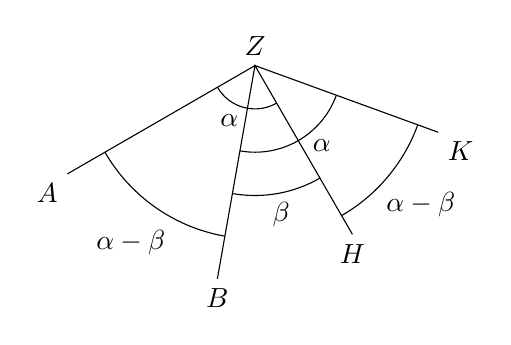
\begin{tikzpicture}[scale=.55]
\coordinate (Z) at (0,0);
\coordinate (A) at (-150:5cm);
\coordinate (B) at (-100:5cm);
\coordinate (H) at (-60:4.5cm);
\coordinate (K) at (-20:4.5cm);
\draw (A) node[below left] {$A$} -- (Z) node[above] {$Z$} -- (B) node[below] {$B$};
\draw (H) node[below] {$H$} -- (Z) -- (K) node[below right] {$K$};
\draw (-150:1cm) arc (-150:-60:1);
\draw (-100:2cm) arc (-100:-20:2);
\draw (-100:3cm) arc (-100:-60:3);
\draw (-150:4cm) arc (-150:-100:4);
\draw (-60:4cm) arc (-60:-20:4);
\node at (-115:1.4) {$\alpha$};
\node at (-50:2.4) {$\alpha$};
\node at (-80:3.5) {$\beta$};
\node at (-40:5) {$\alpha - \beta$};
\node at (-125:5) {$\alpha - \beta$};
\end{tikzpicture}
\caption{$\angle AZB=\angle HZK$}\label{f.compass-relative4}
\end{center}
\end{minipage}
\end{figure}

\enlargethispage{2\baselineskip}

$\triangle ZAB\sim\triangle ZHK$ ya que ambos son triángulos isósceles y hemos demostrado que tienen el mismo ángulo vértice. Si denoto $\overline{HK}$ con $x$, entonces:
\begin{eqnarray*}
\frac{m}{s} &=& \frac{n}{x}\\
x&=&\frac{n}{m}s\,.
\end{eqnarray*}
\end{proof}

%%%%%%%%%%%%%%%%%%%%%%%%%%%%%%%%%%%%%%%%%%%%%%%%%%%%%%%%%%%%%%%

\section{Construcción de la intersección de dos líneas}\label{s.two-lines}

\begin{theorem}
Dadas dos rectas que contienen los segmentos $\overline{AB}, \overline{CD}$, es posible construir su intersección $S$.
\end{theorem}

\begin{proof}
Sean $C',D'$ las reflexiones de $C,D$ alrededor de $\overline{AB}$.
Hay dos casos dependiendo de si $C,D$ se encuentran en el mismo lado de $\overline{AB}$ o en lados diferentes. Denominamos $x=\overline{CS}, c=\overline{CC'}, d=\overline{DD'}, e=\overline{CD}$ como se muestra en las Figs.~\ref{f.compass-intersection1}, \ref{f.compass-intersection2}. Calculamos el valor de $x$ para cada caso.

\begin{figure}%[t]
\begin{center}
\begin{tikzpicture}[scale=.9]
\coordinate (A) at (-4,0);
\coordinate (B) at (2,0);
\coordinate (C) at (-3,2);
\coordinate (D) at (1,-1);
\coordinate (Cp) at (-3,-2);
\coordinate (Dp) at (1,1);
\vertex{A};
\vertex{B};
\node[below] at (A) {$A$};
\node[below] at (B) {$B$};
\node[above] at (C) {$C$};
\node[below] at (D) {$D$};
\node[below] at (Cp) {$C'$};
\node[above] at (Dp) {$D'$};
\draw[name path=ab] ($(A)!1.3!(B)$) -- ($(B)!1.3!(A)$);
\draw[name path=cd] ($(C)!1.2!(D)$) -- ($(D)!1.1!(C)$);
\path [name intersections={of=ab and cd,by={S}}];
\node[above] at (S) {$S$};
\draw (Cp) -- node[below] {$x$} (S);
\draw (S) -- node[above,xshift=-5pt] {$e\!-\!x$} (Dp);
\draw (C) -- node[above left,yshift=6pt] {$c$} (Cp);
\draw (D) -- node[above right,yshift=6pt] {$d$} (Dp);
\path (C) -- node[right,xshift=2pt] {$x$} (S);
\path (S) -- node[left,near end,xshift=-2pt] {$e\!-\!x$} (D);
\node[below left] at (C|-A) {$Z$};
\vertex{C};
\vertex{D};
\vertex{Cp};
\vertex{Dp};
\draw ($(C)!.5!(Cp)$) rectangle +(6pt,6pt);
\draw[rotate=90] ($(D)!.5!(Dp)$) rectangle +(6pt,6pt);
\end{tikzpicture}
\end{center}
\caption{Construcción de la intersección de dos líneas (1)}\label{f.compass-intersection1}
\end{figure}

\textit{Caso 1:}
$C,D$ están en lados distintos de $\overline{AB}$.
$S$ está en $\overline{AB}$ porque $\triangle CZS\cong \triangle C'ZS$ por lado-ángulo-lado: $\overline{CZ}=\overline{C'Z}$, $\angle CZS=\angle C'ZS=90^\circ$ y $\overline{ZS}$ es un lado común. Por tanto $\overline{C'S}=\overline{CS}$ y análogamente $\overline{D'S}=\overline{DS}$. $\triangle CSC'\sim\triangle DSD'$ son semejantes por lo que $\displaystyle\frac{x}{e-x} = \displaystyle\frac{c}{d}$ y resolviendo la ecuación se obtiene $x=\displaystyle\frac{c}{c+d}e$.

\begin{figure}%[b]
\begin{center}
\begin{tikzpicture}[scale=.9]
\coordinate (A) at (-4,0);
\coordinate (B) at (2,0);
\coordinate (C) at (-3,2);
\coordinate (D) at (-1,1);
\coordinate (Cp) at (-3,-2);
\coordinate (Dp) at (-1,-1);
\vertex{A};
\vertex{B};
\node[below] at (A) {$A$};
\node[below] at (B) {$B$};
\node[above] at (C) {$C$};
\node[above] at (D) {$D$};
\node[below] at (Cp) {$C'$};
\node[below] at (Dp) {$D'$};
\draw[name path=ab] ($(A)!1.3!(B)$) -- ($(B)!1.3!(A)$);
\draw[name path=cd] ($(C)!2.2!(D)$) -- ($(D)!1.1!(C)$);
\path [name intersections={of=ab and cd,by={S}}];
\node[above] at (S) {$S$};
\draw (Cp) -- (S);
\draw (C) -- node[above left,yshift=6pt] {$c$} (Cp);
\draw (D) -- node[above right,yshift=6pt] {$d$} (Dp);
\path (C) -- node[above] {$e$} (D);
\path (Cp) -- node[below] {$e$} (Dp);
\path (D) -- node[above right,xshift=-4pt] {$x-e$} (S);
\path (Dp) -- node[below right,xshift=-4pt] {$x-e$} (S);
\node[below left] at (C|-A) {$Z$};
\vertex{C};
\vertex{D};
\vertex{Cp};
\vertex{Dp};
\draw ($(C)!.5!(Cp)$) rectangle +(6pt,6pt);
\draw[rotate=90] ($(D)!.5!(Dp)$) rectangle +(6pt,6pt);
\end{tikzpicture}
\end{center}
\caption{Construcción de la intersección de dos líneas (2)}\label{f.compass-intersection2}
\end{figure}

\begin{figure}
\begin{center}
\begin{tikzpicture}[scale=.8]
\coordinate (A) at (-4,0);
\coordinate (B) at (2,0);
\coordinate (C) at (-3,2);
\coordinate (D) at (1,-1);
\coordinate (Cp) at (-3,-2);
\coordinate (Dp) at (1,1);
\vertex{A};
\vertex{B};
\node[below left] at (A) {$A$};
\node[below] at (B) {$B$};
\node[above] at (C) {$C$};
\node[below] at (D) {$D$};
\node[left] at (Cp) {$C'$};
\node[above] at (Dp) {$D'$};
\draw[name path=ab] ($(A)!1.3!(B)$) -- ($(B)!1.3!(A)$);
\draw[name path=cd] ($(C)!1.2!(D)$) -- ($(D)!1.1!(C)$);
\path [name intersections={of=ab and cd,by={S}}];
\node[above,yshift=4pt] at (S) {$S$};
\draw (Cp) -- node[below right,xshift=5pt,yshift=5pt] {$e$} (Dp);
\path (C) -- node[above left] {$c$} (Cp);
\draw[thick,dashed] (D) -- node[above right] {$d$} (Dp);
\draw[name path=circled] (D) let
  \p1 = ($ (D) - (C) $),
  \n2 = {veclen(\x1,\y1)}
in
  ++(130:\n2) arc (130:230:\n2);

\draw[name path=circlecp] (Cp) let
  \p1 = ($ (D) - (Dp) $),
  \n2 = {veclen(\x1,\y1)}
in
  ++(-180:\n2) arc (-180:0:\n2);
\path [name intersections={of=circled and circlecp,by={H}}];
\node[below left] at (H) {$H$};
\draw ($(C)!1.2!(H)$) -- (C);
\draw (H) -- node[right] {$d$} (Cp);
\draw (D) -- node[right,xshift=18pt,yshift=12pt] {$e$} (H);
\vertex{Cp};
\vertex{D};
\vertex{C};
\vertex{Dp};
\vertex{H};
\path (C) -- node[above] {$x$} (S);
\path (Cp) -- node[below] {$x$} (S);
\end{tikzpicture}
\end{center}
\caption{Construcción de la intersección de dos líneas (3)}\label{f.compass-intersection3}
\end{figure}


\textit{Caso 2:}
$C,D$ están en el mismo lado de $\overline{AB}$. $\triangle CSC'\sim\triangle DSD'$ da $\displaystyle\frac{x}{x-e}=\frac{c}{d}\displaystyle$ y resolviendo la ecuación se obtiene $x=\displaystyle\frac{c}{c-d}e$.

Construimos las circunferencias $c(C',d), c(D,e)$ y denotamos su intersección con $H$ (Fig.~\ref{f.compass-intersection3}). La suma de los segmentos $\overline{CC'}, \overline{C'H}$ es $c + d$. Hay que demostrar que $H$ está en la prolongación de $\overline{CC'}$ para que $\overline{CH}$ sea un segmento de longitud $c+d$. $\overline{CH} = c - d$ en el caso de que $D$ esté en el mismo lado de $\overline{AB}$ que $C$ (no se muestra en el diagrama).

$H$ es la intersección de $c(C',d), c(D,e)$ por lo que $\overline{DH}=e$, $\overline{C'H}=d$. Por construcción $\overline{C'D'} = e$, $\overline{D'D}=d$ por lo que el cuadrilátero $\overline{C'D'DH}$ es un paralelogramo. 

Por construcción $\overline{DD'}\parallel\overline{CC'}$ entonces $\overline{C'H}\parallel \overline{DD'}$ y por tanto $\overline{C'H}\parallel\overline{CC'}$. Como uno de sus extremos es $C'$ debe estar en la recta que contiene a $\overline{CC'}$. Por el Teorema~\ref{thm.add-subtract-mm}, a partir de las longitudes $c,d,e$ se puede construir un segmento de longitud $c+d$ y por el Teorema~\ref{thm.compass-ratio} se puede construir un segmento de longitud $x=\displaystyle\frac{c}{c+d}e$. $S$, la intersección de $c(C',x)$ y $c(C,x)$, es también la intersección de $\overline{AB}, \overline{CD}$ (Fig.~\ref{f.compass-intersection4}).
\end{proof}

\begin{figure}%[t]
\begin{center}
\begin{tikzpicture}[scale=.9]
\coordinate (A) at (-4,0);
\coordinate (B) at (2,0);
\coordinate (C) at (-3,2);
\coordinate (D) at (1,-1);
\coordinate (Cp) at (-3,-2);
\coordinate (Dp) at (1,1);
\vertex{A};
\vertex{B};
\node[below left] at (A) {$A$};
\node[below] at (B) {$B$};
\node[above] at (C) {$C$};
\node[below] at (D) {$D$};
\node[left] at (Cp) {$C'$};
\node[above] at (Dp) {$D'$};
\draw[name path=ab] ($(A)!1.3!(B)$) -- ($(B)!1.3!(A)$);
\draw[name path=cd] ($(C)!1.2!(D)$) -- ($(D)!1.1!(C)$);
\path [name intersections={of=ab and cd,by={S}}];
\node[above,yshift=4pt] at (S) {$S$};
\draw (Cp) -- (Dp);
\path (C) -- node[above,yshift=4pt] {$x$} (S);
\path (Cp) -- node[below,yshift=-4pt] {$x$} (S);
\path (C) -- node[above left] {$c$} (Cp);
\draw (D) -- node[above right] {$d$} (Dp);
\draw[name path=circled] (C) let
  \p1 = ($ (S) - (C) $),
  \n2 = {veclen(\x1,\y1)}
in
  ++(-10:\n2) arc (-10:-100:\n2);

\draw[name path=circlecp] (Cp) let
  \p1 = ($ (S) - (C) $),
  \n2 = {veclen(\x1,\y1)}
in
  ++(100:\n2) arc (100:0:\n2);
\draw (Cp) -- (C);
\vertex{C};
\vertex{Cp};
\vertex{D};
\vertex{Dp};
\end{tikzpicture}
\end{center}
\caption{Construcción de la intersección de dos líneas (4)}\label{f.compass-intersection4}
\end{figure}

%%%%%%%%%%%%%%%%%%%%%%%%%%%%%%%%%%%%%%%%%%%%%%%%%%%%%%%%%%%%%%%

\section[La intersección de una recta y una circunferencia]
{Construcción de la intersección de una recta y una circunferencia}\label{s.line-circle}

\begin{theorem}
Dada una circunferencia $k=C(M,r)$ y una recta $l$ es posible construir las intersecciones de $k$ y $l$.
\end{theorem}

\begin{proof}
Construimos $M'$, la reflexión de $M$ alrededor de $l$ y construimos la circunferencia $k'=c(M',r)$. Como $\triangle MYM'\cong\triangle MXM'$, $X,Y$, los puntos de intersección de $k,k'$, son los puntos de intersección de $l$ y $k$. (Fig.~\ref{f.compass-circle4}).

Esta construcción no puede hacerse si $M$ está sobre la recta $l$. En ese caso se elige un punto arbitrario $A$ sobre $l$ que esté a una distancia mayor que $r$ de $M$. Usando el teorema~\ref{thm.add-subtract-mm} acortamos y alargamos $\overline{AM}$ en $r$. $X,Y$, los puntos extremos de estos segmentos, son las intersecciones de $k$ y $l$ (Fig.~\ref{f.compass-circle5}).
\end{proof}

\begin{figure}%[t]
\begin{center}
\begin{tikzpicture}[scale=.5]
\coordinate (A) at (-7,0);
\coordinate (B) at (8,0);
\coordinate (M) at (0,-2);
\coordinate (Mp) at (0,2);
\node[below left] at (M) {$M$};
\node[above left] at (Mp) {$M'$};
\draw[name path=c1] (M) circle[radius=3cm];
\draw[name path=c2] (Mp) circle[radius=3cm];
\draw[name path=ab] ($(A)!1.2!(B)$) --
  node[above,very near end] {$l$} ($(B)!1.2!(A)$);
\path [name intersections={of=c1 and c2,by={S1,S2}}];
\path[name path=radius1] (M) -- ++(15:4cm);
\path [name intersections={of=c1 and radius1,by={R1}}];
\draw (M) -- node[below] {$r$} (R1);
\path[name path=radius2] (Mp) -- ++(40:4cm);
\path [name intersections={of=c2 and radius2,by={R2}}];
\draw (Mp) -- node[above] {$r$} (R2);
\draw (Mp) -- (M) -- (S1) -- (Mp) -- (S2) -- (M);
\node[right,xshift=6pt,yshift=6pt] at (S1) {$X$};
\node[left,xshift=-6pt,yshift=6pt] at (S2) {$Y$};
\draw (0,0) rectangle +(10pt,10pt);
\node at (-3.5,-3) {$k$};
\node at (-3.5,3) {$k'$};
\end{tikzpicture}
\end{center}
\caption{Construcción de la intersección de una recta y una circunferencia (1)}\label{f.compass-circle4}
\end{figure}


\begin{figure}%[t]
\begin{center}
\begin{tikzpicture}[scale=.5]
\coordinate (A) at (-7,0);
\coordinate (B) at (8,0);
\coordinate (M) at (0,0);
\vertex{M};
\vertex{A};
\node[below] at (A) {$A$};
\node[below left] at (M) {$M$};
\draw[name path=c1] (M) circle[radius=3cm];
\draw[name path=ab] ($(A)!1.2!(B)$) -- 
  node[above,very near end] {$l$} ($(B)!1.2!(A)$);
\path[name path=radius1] (M) -- ++(50:4cm);
\path [name intersections={of=c1 and radius1,by={R1}}];
\draw (M) -- node[above] {$r$} (R1);
\path [name intersections={of=c1 and ab,by={S1,S2}}];
\node[above right] at (S1) {$X$};
\node[above left] at (S2) {$Y$};
\path (M) -- node[below,xshift=4pt] {$\overline{AM}+r$} (S1);
\path (A) -- node[below] {$\overline{AM}-r$} (S2);
\node at (-2.5,2.5) {$k$};
\end{tikzpicture}
\end{center}
\caption{Construcción de la intersección de una recta y una circunferencia (2)}\label{f.compass-circle5}
\end{figure}


\subsection*{¿Cuál es la sorpresa?}

Cuando se aprende a construir con regla y compás, es obvio que ambas herramientas son necesarias. Por lo tanto, fue toda una sorpresa descubrir que un compás es suficiente. La demostración es bastante larga, así que no vamos a dejar la regla en casa, pero el teorema demuestra que no debemos suponer que no existen alternativas a conceptos matemáticos bien conocidos.

\subsection*{Fuentes}

Este capítulo se basa en el problema $33$ de \cite{dorrie1} reelaborado por Michael Woltermann \cite{dorrie2}. Una demostración adicional se puede encontrar en \cite{mm}.
